\chapter{Finding Ground Truth for a Mobile Platform}
The image code written in Open CV was not just for use with object detection for the manipulator. The first Open CV code for color detection was used in a program to calculate the ground truth, or path traveled, by a mobile platform from an overhead video. The first object recognition code works for this purpose because the environment for these tests was controlled, meaning the robot was the only object of a color in the video. The ground truth is important to have so that it can be compared to results of path reconstruction based on sensors on the robot.

For this situation a red rectangle was placed on top of the platform and video taken from above the test area using a GoPro camera. Loading the video file into the open CV program after. The video was analyzed one frame at a time to locate the robot and record its center position. The colored rectangle was positioned on the robot in such a way that the center of the rectangle was also the center of the robot.
 
\section{First Solution}
Unlike with the color tracking using the depth camera the pixel coordinate of the desired location is not enough to get a estimate of the real world xyz position of the point as there is no depth data. It was therefore necessary to find another way to accurately measure the world coordinates of the robots center. The first method tried for this was using a least squares method to derive a linear equation to convert between pixel and world coordinates. The world coordinates were only calculated as an xy point as the robot traveled across a smooth surface and the z value was constant. A set of about 20 points were taken from the image at points where the world coordinates were known. Since the floor of the test area had tiles of a known size so the corners were used as the known points. 

The conversion was setup as y = Ax+B where y is the vector of real world xy coordinates, x is the pixel uv values, and A and B were matrices found using least squares. The matrix $\tilde{A}$ which equals $[A|B]$ was solved by $YX(XX^T)^{-1}$ where $XX^T$ is an invertible matrix and Y and X are full of known conversion points. These calculations were done to find A and B in Matlab and then put into the path finding code to convert to world coordinates.

This method had a number of problems; mainly inaccuracy and manual work. The linear system calculated did not provide a good estimate for converting to world coordinates. At times the result was eight inches from the actual xy coordinate. The desired accuracy range was to be with two inches of the actual value. Each time a new data was acquired the A and B matrices had to be recalculated. This is because the camera's position changes enough each time it was mounted above the test area to make the old matrices unusable. This meant that for each new run points would need to be found by hand to resolve for the A B matrices before being able to run the tracking program.

\section{Second Solution}

To address these issues the first step was to mount the GoPro in such a way that its positioning in the test area was always the same, or at very least close enough to the same to produce a manageable error. The mount that comes with the GoPro has multiple bendable joints so even if mounted at the same location the camera is not likely to be in the same orientation. A more stationary mount for the GoPro was designed in Solidworks. The design was to have a case to hold the GoPro which was attached to a clip that fit around the overhead light in the test area. The point at which the clip attached to the light was marked on the light and allowed the camera to be mounted at the same height and angle for all test runs in the environment. Figure \ref{fig:mount} shows the Solidworks model for this mount which was then 3D printed and used to hold the camera.

\begin{figure}[h]
\centering
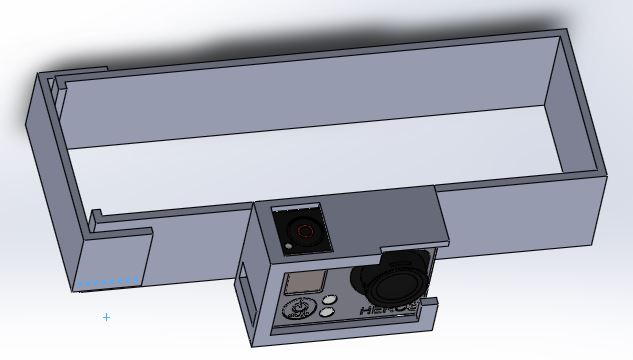
\includegraphics[width=0.5\textwidth]{camera}
\caption{Solidworks model of GoPro mount.}
\label{fig:mount}
\end{figure}

With the camera in a fixed location a more accurate way to convert the pixel coordinates to world coordinates was developed. To account for the changes in position caused by the height of the mobile platform about thirty-five data points were gathered to convert the center of an objects pixel coordinates to the real world coordinates. The object used for this was the same height was the robot to create the same offset. This offset can be seen in Figure \ref{fig:offset}. The bottle was placed at the corner of four tiles yet since the camera is not directly above it the object's center does not appear to be at the corner. The first version of the code did not account for this distortion and added to its inaccuracy. 

\begin{figure}[h]
    \centering
    \begin{subfigure}[b]{0.45\textwidth}
    	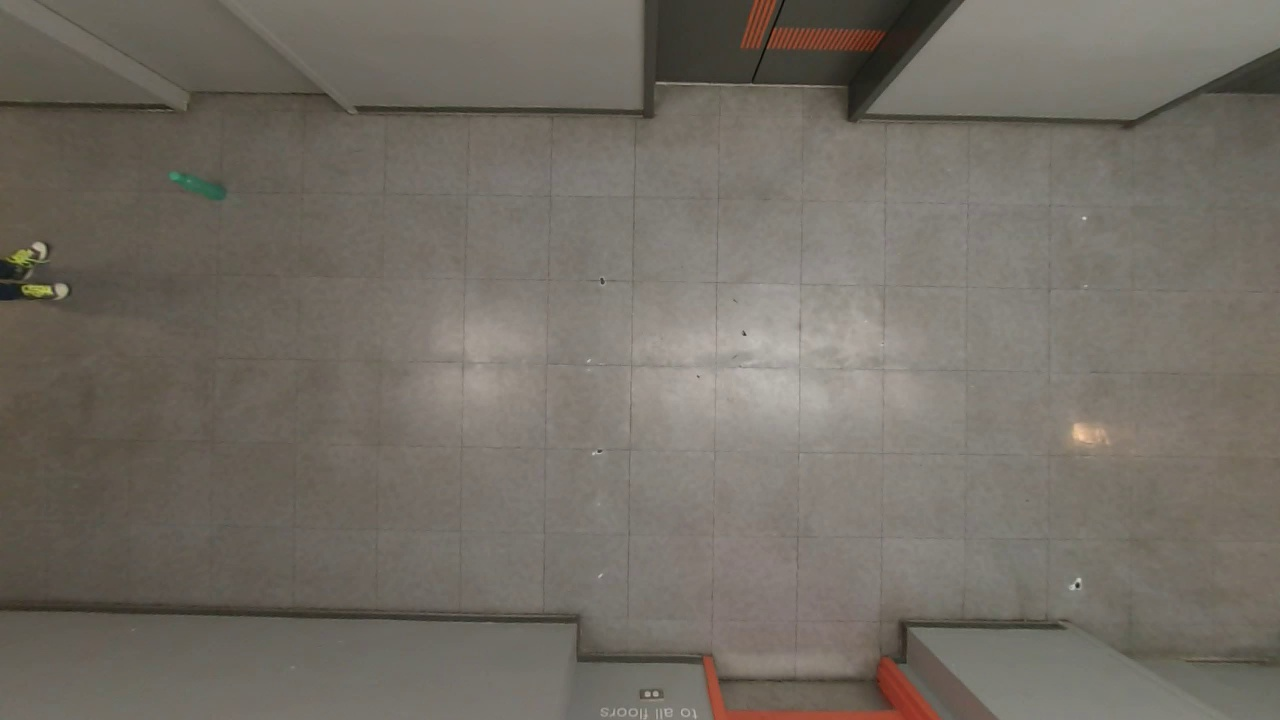
\includegraphics[width=\textwidth]{testArea}
    	\caption{Demonstration of 3D object offset. }
    	\label{fig:offset}
   	 \end{subfigure}
   	 \quad
    \begin{subfigure}[b]{0.45\textwidth}
		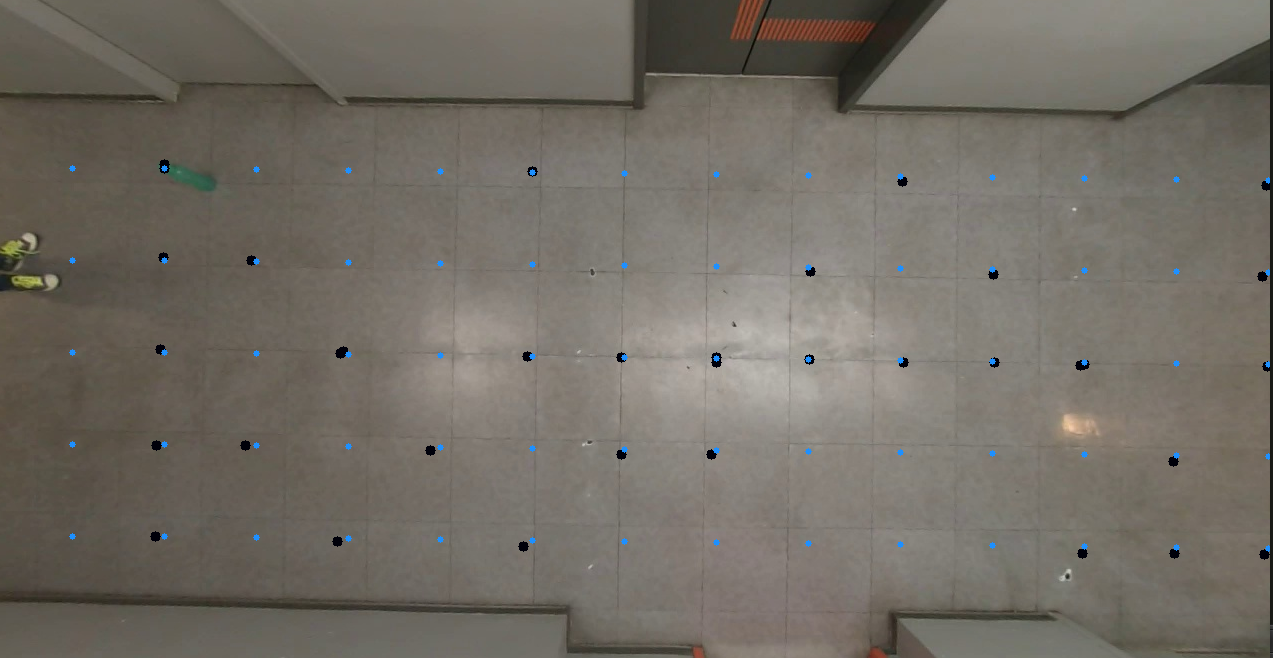
\includegraphics[width=\textwidth]{newcodepoints}
		\caption{Generated points versus manually found points. }
		\label{fig:genpoints}
    \end{subfigure}
    \quad %add desired spacing between images, e. g. ~, \quad, \qquad, \hfill etc.
      %(or a blank line to force the subfigure onto a new line)
 	\caption{View of test area from GoPro.}
 	\label{fig:images}
\end{figure}

An equation was made to generate the x and y world coordinates, The x-coordinate equation was linear and only dependent on the corresponding u pixel value. The y coordinate equation was a function of both the u and v pixel coordinates. This is because the lines found for the tiles were not perpendicular as the horizontal lines sloped slightly upwards making the y calculations a function of both x and y. A lookup table was generated for each tile corder in the test area based on these equations. Figure \ref{fig:genpoints} shows the generated points, in black, compared to those hand gathered, in blue. The lookup table could then be implemented in the main path locating program to convert to world coordinates. 

The results of this program were more accurate, within about 2 inches of the actual location, which was the desired accuracy. It was also no longer necessary to recalculate formulas for each new test in the environment. An example of the generated path is shown in Figure \ref{fig:path}. There is some jitters in the found path due to the color detection not creating the ideal data. Low pass filtering does improve the path making it smother, but there is still some inaccuracy. 

\begin{figure}
\centering
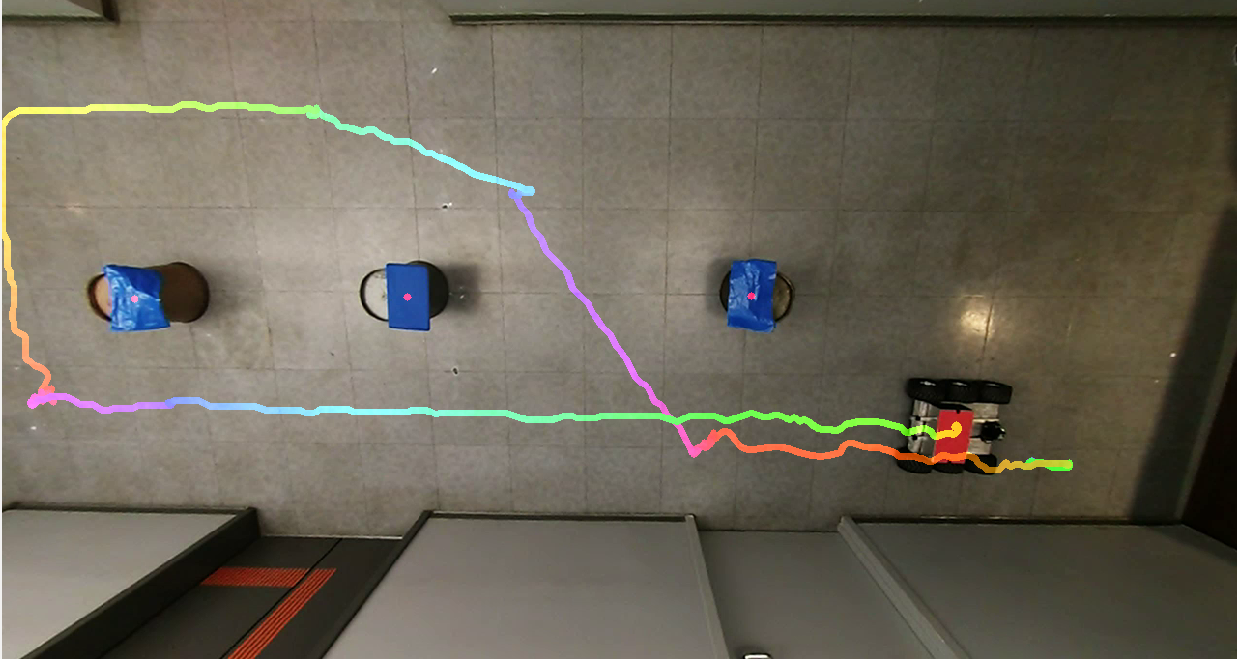
\includegraphics[width=0.5\textwidth]{path}
\caption{Found path of mobile platform drawn on camera image.}
\label{fig:path}
\end{figure}